\documentclass[aspectratio=169]{beamer}

% ── Theme and Colors ──────────────────────────────────────
\usetheme{default}
\usecolortheme{default}
\usefonttheme{serif}
\setbeamertemplate{navigation symbols}{}
\setbeamertemplate{footline}[frame number]

% ── Packages ──────────────────────────────────────────────
\usepackage[T1]{fontenc}
\usepackage{graphicx}
\usepackage{xcolor}
\usepackage{tikz}
\usetikzlibrary{arrows.meta,positioning,shapes.geometric,fit,calc,
                decorations.pathreplacing,backgrounds,patterns}
\usepackage{booktabs}
\usepackage{tabularx}
\usepackage{amsmath,amssymb}
\usepackage{multimedia}

% ── Brand Colors ──────────────────────────────────────────
\definecolor{garnet}{HTML}{73000A}
\definecolor{rose}{HTML}{CC2E40}
\definecolor{atlantic}{HTML}{466A9F}
\definecolor{congaree}{HTML}{1F414D}
\definecolor{horseshoe}{HTML}{65780B}
\definecolor{grass}{HTML}{CED318}
\definecolor{honeycomb}{HTML}{A49137}
\definecolor{warmgrey}{HTML}{676156}
\definecolor{sandstorm}{HTML}{FFF2E3}
\definecolor{bk90}{HTML}{363636}
\definecolor{bk70}{HTML}{5C5C5C}
\definecolor{bk50}{HTML}{A2A2A2}
\definecolor{bk30}{HTML}{C7C7C7}
\definecolor{bk10}{HTML}{ECECEC}

% ── Beamer Colors ─────────────────────────────────────────
\setbeamercolor{title}{fg=garnet}
\setbeamercolor{frametitle}{fg=garnet}
\setbeamercolor{structure}{fg=garnet}
\setbeamercolor{item}{fg=garnet}
\setbeamercolor{block title}{bg=garnet,fg=white}
\setbeamercolor{block body}{bg=bk10}
\setbeamercolor{alerted text}{fg=rose}

% ── TikZ Styles ───────────────────────────────────────────
\tikzset{
  pipeblock/.style={
    rectangle, draw=#1, fill=#1!10, thick,
    minimum width=2.0cm, minimum height=0.8cm,
    font=\small\sffamily, align=center, inner sep=4pt
  },
  pipeblock/.default=garnet,
  dataarrow/.style={
    -{Stealth[length=5pt]}, thick, color=#1
  },
  dataarrow/.default=bk70,
  labelnode/.style={
    font=\scriptsize\sffamily, color=bk70
  },
  eqbox/.style={
    rectangle, draw=#1, fill=#1!5, thick,
    font=\small, align=center, inner sep=6pt
  },
  eqbox/.default=atlantic,
}

% ══════════════════════════════════════════════════════════
\title{\textcolor{garnet}{\textbf{Metric3D v2}}}
\subtitle{A Versatile Monocular Geometric Foundation Model\\for Zero-Shot Metric Depth and Surface Normal Estimation}
\author{Presented by J.C.\ Vaught}
\institute{CSCE 763 --- Digital Image Processing\\University of South Carolina}
\date{Spring 2026}

\begin{document}

% ══════════════════════════════════════════════════════════
% SLIDE 0: Title
% ══════════════════════════════════════════════════════════
\begin{frame}
\titlepage
\vspace{-0.5cm}
\centering
{\footnotesize Mu Hu, Wei Yin, Chi Zhang, Zhipeng Cai, Xiao Long, Hao Chen,\\
Kaixuan Wang, Gang Yu, Chunhua Shen, Shaojie Shen\\[4pt]
\textit{IEEE TPAMI}, Vol.\ 46, No.\ 12, 2024}
\end{frame}

% ══════════════════════════════════════════════════════════
\section{Introduction \& Background}
% ══════════════════════════════════════════════════════════

% ── SLIDE 1: Hook ─────────────────────────────────────────
\begin{frame}{What Can You Measure from a Single Photo?}
\begin{columns}[T]
\column{0.55\textwidth}
\textbf{Goal:} From one RGB image, recover per-pixel
\begin{itemize}
  \item \textcolor{atlantic}{\textbf{Metric depth}} --- distance in meters from camera to each point
  \item \textcolor{congaree}{\textbf{Surface normals}} --- 3D orientation of each surface patch
\end{itemize}

\vspace{0.4cm}
\textbf{Connection to course:} The pinhole camera model (Ch.\ 2) relates 3D world coordinates to 2D image coordinates via focal length $f$:
\[
  u = f\,\frac{X}{Z}, \qquad v = f\,\frac{Y}{Z}
\]

Without knowing $f$, depth is ambiguous.

\column{0.42\textwidth}
% Placeholder for campus photo + depth/normal output
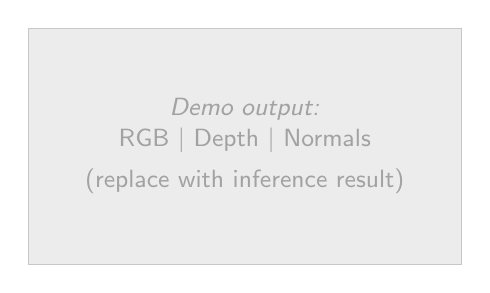
\begin{tikzpicture}
  \node[rectangle, draw=bk30, fill=bk10, minimum width=5.5cm, minimum height=3.0cm,
        font=\small\sffamily\color{bk50}, align=center] {
    \textit{Demo output:}\\RGB $\mid$ Depth $\mid$ Normals\\[4pt]
    (replace with inference result)
  };
\end{tikzpicture}
\end{columns}
\end{frame}

% ── SLIDE 2: Metric Ambiguity ─────────────────────────────
\begin{frame}{Why Is This Hard? --- Metric Ambiguity}
\begin{columns}[T]
\column{0.52\textwidth}
\textbf{Key insight:} Two cameras with different focal lengths can produce \textit{identical} images of a scene at different depths.

\vspace{0.3cm}
The apparent depth scales with focal length:
\[
  \boxed{d_a = \hat{S} \cdot \frac{\hat{f}}{\hat{S}'}}
\]

where $\hat{S}$ is real-world size, $\hat{f}$ is focal length, and $\hat{S}'$ is projected size.

\vspace{0.3cm}
A network trained on mixed datasets with different cameras sees \textbf{conflicting depth labels} for visually identical patches.

\column{0.45\textwidth}
% Animation placeholder -- replace with metric_ambiguity.gif
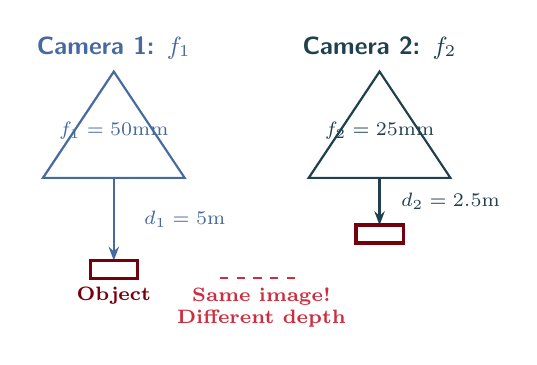
\begin{tikzpicture}[scale=0.75]
  % Camera 1
  \node[font=\small\sffamily\bfseries, color=atlantic] at (0,4.2) {Camera 1: $f_1$};
  \draw[thick, atlantic] (0,3.8) -- (-1.2,2.0) -- (1.2,2.0) -- cycle;
  \node[font=\scriptsize, color=atlantic] at (0,2.8) {$f_1 = 50$mm};
  \draw[dataarrow=atlantic] (0,2.0) -- (0,0.6);
  \node[font=\scriptsize, color=atlantic] at (1.2,1.3) {$d_1 = 5$m};

  % Object
  \draw[very thick, garnet] (-0.4,0.3) rectangle (0.4,0.6);
  \node[font=\scriptsize\bfseries, color=garnet] at (0,0.0) {Object};

  % Camera 2
  \node[font=\small\sffamily\bfseries, color=congaree] at (4.5,4.2) {Camera 2: $f_2$};
  \draw[thick, congaree] (4.5,3.8) -- (3.3,2.0) -- (5.7,2.0) -- cycle;
  \node[font=\scriptsize, color=congaree] at (4.5,2.8) {$f_2 = 25$mm};
  \draw[dataarrow=congaree] (4.5,2.0) -- (4.5,1.2);
  \node[font=\scriptsize, color=congaree] at (5.7,1.6) {$d_2 = 2.5$m};

  % Object 2
  \draw[very thick, garnet] (4.1,0.9) rectangle (4.9,1.2);

  % Same projection
  \draw[thick, dashed, rose] (1.8,0.3) -- (3.2,0.3);
  \node[font=\scriptsize\bfseries, color=rose, align=center] at (2.5,-0.2) {Same image!\\Different depth};
\end{tikzpicture}
\end{columns}
\end{frame}

% ── SLIDE 3: Taxonomy ─────────────────────────────────────
\begin{frame}{Depth Estimation Taxonomy}
\centering
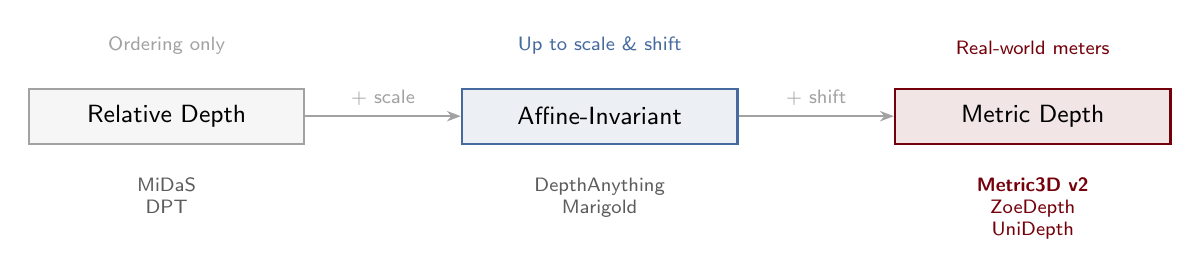
\begin{tikzpicture}[
  taxbox/.style={rectangle, draw=#1, fill=#1!10, thick,
    minimum height=0.7cm, font=\small\sffamily, align=center, inner sep=5pt},
  taxbox/.default=bk70
]
  % Levels
  \node[taxbox=bk50, minimum width=3.5cm] (rel) at (0,0) {Relative Depth};
  \node[taxbox=atlantic, minimum width=3.5cm] (aff) at (5.5,0) {Affine-Invariant};
  \node[taxbox=garnet, minimum width=3.5cm] (met) at (11,0) {Metric Depth};

  % Arrows
  \draw[dataarrow=bk50] (rel.east) -- (aff.west)
    node[midway, above, font=\scriptsize\sffamily] {+ scale};
  \draw[dataarrow=bk50] (aff.east) -- (met.west)
    node[midway, above, font=\scriptsize\sffamily] {+ shift};

  % Methods
  \node[font=\scriptsize\sffamily, color=bk70, below=0.3cm of rel, align=center] {MiDaS\\DPT};
  \node[font=\scriptsize\sffamily, color=bk70, below=0.3cm of aff, align=center] {DepthAnything\\Marigold};
  \node[font=\scriptsize\sffamily, color=garnet, below=0.3cm of met, align=center] {\textbf{Metric3D v2}\\ZoeDepth\\UniDepth};

  % Descriptions
  \node[font=\scriptsize\sffamily, color=bk50, above=0.3cm of rel] {Ordering only};
  \node[font=\scriptsize\sffamily, color=atlantic, above=0.3cm of aff] {Up to scale \& shift};
  \node[font=\scriptsize\sffamily, color=garnet, above=0.3cm of met] {Real-world meters};
\end{tikzpicture}

\vspace{0.5cm}
\textbf{Metric3D v2} achieves \textit{zero-shot metric depth} by explicitly modeling camera intrinsics, unlike methods that learn only relative ordering.
\end{frame}

% ══════════════════════════════════════════════════════════
\section{Methodology}
% ══════════════════════════════════════════════════════════

% ── SLIDE 4: Architecture Overview ────────────────────────
\begin{frame}{Architecture Overview}
\centering
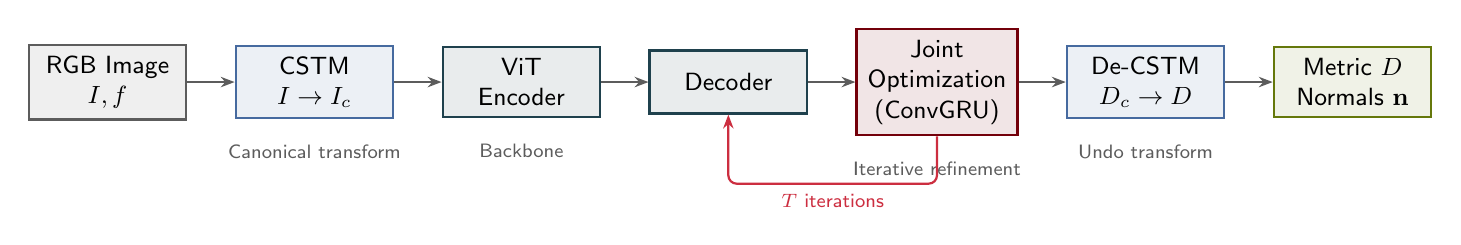
\begin{tikzpicture}[node distance=0.6cm]
  % Nodes
  \node[pipeblock=bk70] (input) {RGB Image\\$I, f$};
  \node[pipeblock=atlantic, right=of input] (cstm) {CSTM\\$I \to I_c$};
  \node[pipeblock=congaree, right=of cstm] (enc) {ViT\\Encoder};
  \node[pipeblock=congaree, right=of enc] (dec) {Decoder};
  \node[pipeblock=garnet, right=of dec] (gru) {Joint\\Optimization\\(ConvGRU)};
  \node[pipeblock=atlantic, right=of gru] (decstm) {De-CSTM\\$D_c \to D$};
  \node[pipeblock=horseshoe, right=of decstm] (out) {Metric $D$\\Normals $\mathbf{n}$};

  % Arrows
  \draw[dataarrow] (input) -- (cstm);
  \draw[dataarrow] (cstm) -- (enc);
  \draw[dataarrow] (enc) -- (dec);
  \draw[dataarrow] (dec) -- (gru);
  \draw[dataarrow] (gru) -- (decstm);
  \draw[dataarrow] (decstm) -- (out);

  % Labels
  \node[labelnode, below=0.2cm of cstm] {Canonical transform};
  \node[labelnode, below=0.2cm of enc] {Backbone};
  \node[labelnode, below=0.2cm of gru] {Iterative refinement};
  \node[labelnode, below=0.2cm of decstm] {Undo transform};

  % Feedback loop
  \draw[dataarrow=rose, rounded corners=3pt]
    (gru.south) -- ++(0,-0.6) -| (dec.south)
    node[pos=0.25, below, font=\scriptsize\sffamily, color=rose] {$T$ iterations};
\end{tikzpicture}

\vspace{0.4cm}
\begin{itemize}
  \item \textbf{Modular:} Any backbone (ViT-S, ViT-L, ViT-G) plugs in; CSTM is backbone-agnostic
  \item \textbf{Two key innovations:} Canonical Camera Space Transform (CSTM) and Joint Depth-Normal Optimization
\end{itemize}
\end{frame}

% ── SLIDE 5: Focal Length Is Everything ───────────────────
\begin{frame}{Focal Length Is Everything}
\begin{columns}[T]
\column{0.55\textwidth}
The paper establishes two critical observations:

\vspace{0.3cm}
\textbf{O1: Sensor/pixel size does not matter.}\\
Only the ratio of focal length to pixel size matters, and this is captured by the focal length in pixels $f_{\text{px}}$.

\vspace{0.3cm}
\textbf{O2: Focal length is vital for metric depth.}\\
Different focal lengths cause different depth scales. The network must compensate, or depth predictions collapse across diverse cameras.

\vspace{0.3cm}
\textbf{Normals are metric-agnostic:}\\
Surface normals depend only on local geometry, not on absolute depth scale. This makes them an ideal auxiliary signal.

\column{0.42\textwidth}
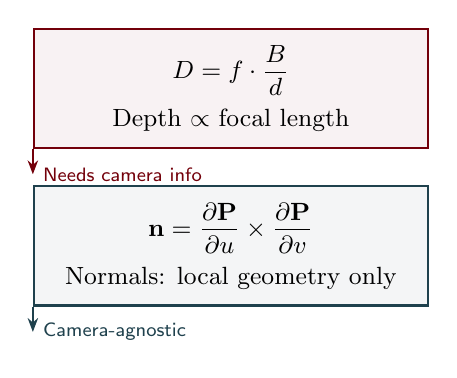
\begin{tikzpicture}[scale=0.8]
  % Depth depends on f
  \node[eqbox=garnet, minimum width=5cm] (deq) at (0,3) {
    $D = f \cdot \dfrac{B}{d}$\\[4pt]
    Depth $\propto$ focal length
  };

  % Normal does not
  \node[eqbox=congaree, minimum width=5cm] (neq) at (0,0.5) {
    $\mathbf{n} = \dfrac{\partial \mathbf{P}}{\partial u} \times \dfrac{\partial \mathbf{P}}{\partial v}$\\[4pt]
    Normals: local geometry only
  };

  \draw[dataarrow=garnet] (deq.south west) -- ++(0,-0.4)
    node[right, font=\scriptsize\sffamily, color=garnet] {Needs camera info};
  \draw[dataarrow=congaree] (neq.south west) -- ++(0,-0.4)
    node[right, font=\scriptsize\sffamily, color=congaree] {Camera-agnostic};
\end{tikzpicture}
\end{columns}
\end{frame}

% ── SLIDE 6: CSTM (Label) ────────────────────────────────
\begin{frame}{Canonical Camera Space Transform --- Label Space}
\begin{columns}[T]
\column{0.55\textwidth}
\textbf{Idea:} Map all training data to a ``canonical'' camera with fixed focal length $f^c = 1000\,\text{px}$.

\vspace{0.3cm}
\textbf{CSTM\textsubscript{label}} transforms depth annotations:
\[
  \boxed{D_c^{*} = \omega_d \cdot D^{*}, \qquad \omega_d = \frac{f^c}{f}}
\]

If $f < f^c$: depth is \textit{scaled up} (wide-angle cameras see closer).\\
If $f > f^c$: depth is \textit{scaled down}.

\vspace{0.3cm}
At inference, \textbf{De-CSTM} reverses:
\[
  D = \frac{D_c}{\omega_d} = D_c \cdot \frac{f}{f^c}
\]

\column{0.42\textwidth}
% Animation placeholder -- replace with cstm_pipeline.gif
\centering
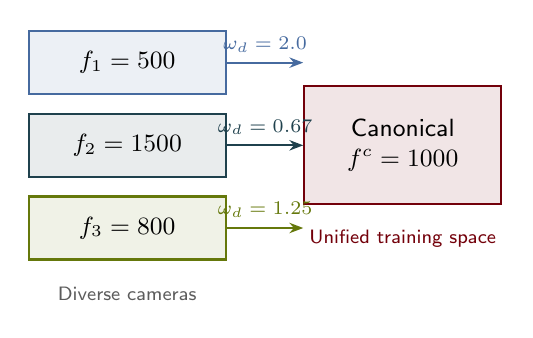
\begin{tikzpicture}[scale=0.7, every node/.style={font=\small\sffamily}]
  % Source cameras
  \node[pipeblock=atlantic, minimum width=2.5cm] (c1) at (0,4) {$f_1 = 500$};
  \node[pipeblock=congaree, minimum width=2.5cm] (c2) at (0,2.5) {$f_2 = 1500$};
  \node[pipeblock=horseshoe, minimum width=2.5cm] (c3) at (0,1.0) {$f_3 = 800$};

  % Canonical
  \node[pipeblock=garnet, minimum width=2.5cm, minimum height=1.5cm] (cc) at (5,2.5)
    {Canonical\\$f^c = 1000$};

  % Arrows with scale factors
  \draw[dataarrow=atlantic] (c1.east) -- (cc.west |- c1)
    node[midway, above, font=\scriptsize] {$\omega_d = 2.0$};
  \draw[dataarrow=congaree] (c2.east) -- (cc.west)
    node[midway, above, font=\scriptsize] {$\omega_d = 0.67$};
  \draw[dataarrow=horseshoe] (c3.east) -- (cc.west |- c3)
    node[midway, above, font=\scriptsize] {$\omega_d = 1.25$};

  % Label
  \node[font=\scriptsize\sffamily, color=bk70] at (0,-0.2) {Diverse cameras};
  \node[font=\scriptsize\sffamily, color=garnet] at (5,0.8) {Unified training space};
\end{tikzpicture}
\end{columns}
\end{frame}

% ── SLIDE 7: CSTM (Image) ────────────────────────────────
\begin{frame}{Canonical Camera Space Transform --- Image Space}
\begin{columns}[T]
\column{0.55\textwidth}
\textbf{CSTM\textsubscript{image}} resizes the input image instead of scaling labels:
\[
  \boxed{I_c = \mathcal{T}(I,\; \omega_r), \qquad \omega_r = \frac{f^c}{f}}
\]

\textbf{Why resize?} After resizing, objects in $I_c$ appear at the angular size they would subtend through the canonical camera. The encoder sees a consistent ``canonical viewpoint.''

\vspace{0.3cm}
\textbf{Both paths are equivalent:}
\begin{itemize}
  \item CSTM\textsubscript{label}: scale depth labels, keep images
  \item CSTM\textsubscript{image}: resize images, keep depth labels
\end{itemize}

In practice, the paper uses \textbf{CSTM\textsubscript{image}} during training.

\column{0.42\textwidth}
\centering
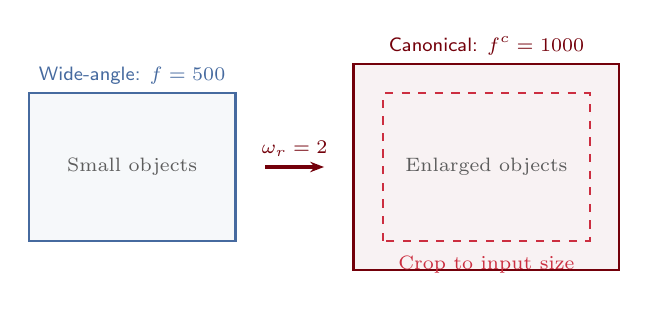
\begin{tikzpicture}[scale=0.75]
  % Original image (wide-angle)
  \draw[thick, atlantic, fill=atlantic!5] (0,3) rectangle (3.5,5.5);
  \node[font=\scriptsize\sffamily, color=atlantic] at (1.75,5.8) {Wide-angle: $f = 500$};
  \node[font=\scriptsize, color=bk70] at (1.75,4.25) {Small objects};

  % Arrow
  \draw[dataarrow=garnet, very thick] (4.0,4.25) -- (5.0,4.25)
    node[midway, above, font=\scriptsize\sffamily] {$\omega_r = 2$};

  % Canonical image (zoomed)
  \draw[thick, garnet, fill=garnet!5] (5.5,2.5) rectangle (10.0,6.0);
  \node[font=\scriptsize\sffamily, color=garnet] at (7.75,6.3) {Canonical: $f^c = 1000$};
  \node[font=\scriptsize, color=bk70] at (7.75,4.25) {Enlarged objects};

  % Crop indicator
  \draw[dashed, rose, thick] (6.0,3.0) rectangle (9.5,5.5);
  \node[font=\scriptsize, color=rose] at (7.75,2.6) {Crop to input size};
\end{tikzpicture}
\end{columns}
\end{frame}

% ── SLIDE 8: Joint Optimization ───────────────────────────
\begin{frame}{Joint Depth-Normal Optimization}
\begin{columns}[T]
\column{0.55\textwidth}
\textbf{Novel contribution:} First method to jointly optimize metric depth and surface normals through an iterative process.

\vspace{0.3cm}
\textbf{ConvGRU iterative refinement:}
\begin{enumerate}
  \item Decoder produces initial coarse estimates $D_0$, $\mathbf{n}_0$
  \item At each iteration $t$:
    \begin{itemize}
      \item Compute update $\Delta_t$ from hidden state
      \item $D_{t+1} = D_t + \Delta_{D,t}$
      \item $\mathbf{n}_{t+1} = \mathbf{n}_t + \Delta_{\mathbf{n},t}$
    \end{itemize}
  \item After $T$ steps: final refined output
\end{enumerate}

\vspace{0.2cm}
\textbf{Why jointly?} Depth and normals are geometrically coupled. Sharing a hidden state lets each task inform the other.

\column{0.42\textwidth}
% Animation placeholder -- replace with convgru_refinement.gif
\centering
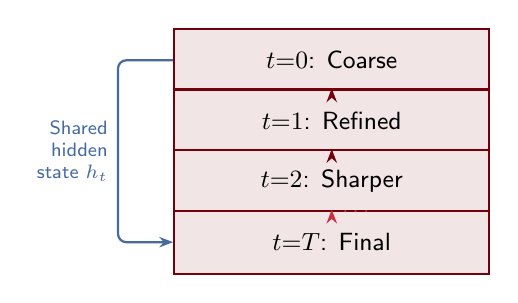
\begin{tikzpicture}[scale=0.7]
  % Iteration blocks
  \foreach \i/\label/\desc in {0/t{=}0/Coarse, 1/t{=}1/Refined, 2/t{=}2/Sharper, 3/t{=}T/Final} {
    \pgfmathsetmacro{\y}{3.5 - \i*1.1}
    \node[pipeblock=garnet, minimum width=4cm] (iter\i) at (3, \y) {\small $\label$: \desc};
  }

  % Arrows
  \draw[dataarrow=garnet] (iter0) -- (iter1);
  \draw[dataarrow=garnet] (iter1) -- (iter2);
  \draw[dataarrow=rose, dashed] (iter2) -- (iter3)
    node[midway, right, font=\scriptsize\sffamily, color=rose] {$\cdots$};

  % Hidden state
  \draw[dataarrow=atlantic, thick, rounded corners=3pt]
    (iter0.west) -- ++(-1,0) |- (iter3.west)
    node[pos=0.25, left, font=\scriptsize\sffamily, color=atlantic, align=right] {Shared\\hidden\\state $h_t$};
\end{tikzpicture}
\end{columns}
\end{frame}

% ── SLIDE 9: Joint Optimization (Losses) ─────────────────
\begin{frame}{Joint Optimization --- Three Supervision Sources}
\centering
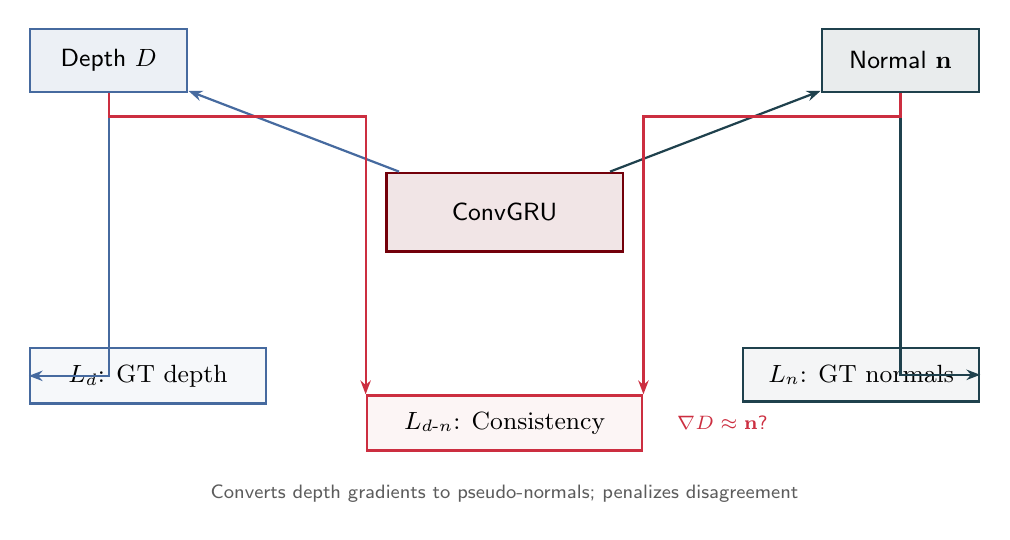
\begin{tikzpicture}[node distance=0.8cm]
  % Central node
  \node[pipeblock=garnet, minimum width=3cm, minimum height=1cm] (gru) {ConvGRU};

  % Depth branch
  \node[pipeblock=atlantic, above left=1.0cm and 2.5cm of gru] (depth) {Depth $D$};
  \node[pipeblock=congaree, above right=1.0cm and 2.5cm of gru] (normal) {Normal $\mathbf{n}$};

  % Loss nodes
  \node[eqbox=atlantic, below left=1.2cm and 1.5cm of gru, minimum width=3cm] (ldepth)
    {$L_d$: GT depth};
  \node[eqbox=congaree, below right=1.2cm and 1.5cm of gru, minimum width=3cm] (lnormal)
    {$L_n$: GT normals};
  \node[eqbox=rose, below=1.8cm of gru, minimum width=3.5cm] (lcons)
    {$L_{d\text{-}n}$: Consistency};

  % Arrows
  \draw[dataarrow=atlantic] (gru) -- (depth);
  \draw[dataarrow=congaree] (gru) -- (normal);
  \draw[dataarrow=atlantic] (depth) |- (ldepth);
  \draw[dataarrow=congaree] (normal) |- (lnormal);
  \draw[dataarrow=rose] (depth.south) -- ++(0,-0.3) -| (lcons.north west);
  \draw[dataarrow=rose] (normal.south) -- ++(0,-0.3) -| (lcons.north east);

  % Annotation
  \node[font=\scriptsize\sffamily, color=rose, right=0.3cm of lcons] {
    $\nabla D \approx \mathbf{n}$?
  };
  \node[font=\scriptsize\sffamily, color=bk70, below=0.3cm of lcons] {
    Converts depth gradients to pseudo-normals; penalizes disagreement
  };
\end{tikzpicture}

\vspace{0.3cm}
\textbf{Key insight:} Only $\sim$20K outdoor images have GT normals. The consistency loss $L_{d\text{-}n}$ lets the model learn normals from depth-only datasets by enforcing geometric agreement.
\end{frame}

% ── SLIDE 10: RPNL ───────────────────────────────────────
\begin{frame}{Random Proposal Normalization Loss (RPNL)}
\begin{columns}[T]
\column{0.55\textwidth}
\textbf{Problem:} Standard depth losses normalize globally. Close objects dominate; distant detail is lost.

\vspace{0.2cm}
\textbf{Analogy from course:} This is the same problem \textit{adaptive histogram equalization} solves for image contrast. Global normalization washes out local structure.

\vspace{0.3cm}
\textbf{RPNL solution:}
\begin{enumerate}
  \item Randomly crop $K$ patches from the depth map
  \item Normalize depth within each patch independently
  \item Compute loss per patch, then average
\end{enumerate}

\vspace{0.2cm}
This forces the network to preserve \textit{local} depth structure everywhere, not just near the camera.

\column{0.42\textwidth}
% Animation placeholder -- replace with rpnl_animation.gif
\centering
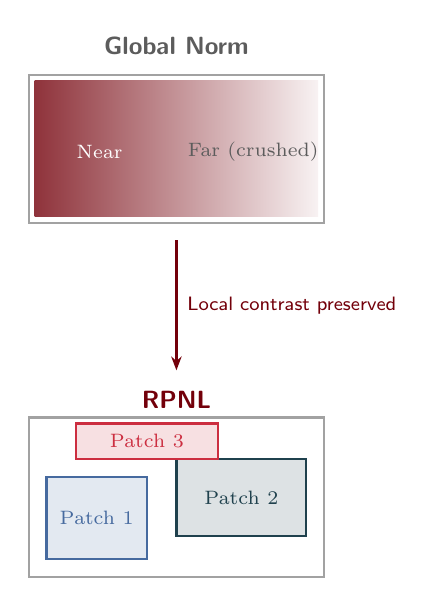
\begin{tikzpicture}[scale=0.75]
  % Global normalization
  \node[font=\small\sffamily\bfseries, color=bk70] at (2.5,5.5) {Global Norm};
  \draw[thick, bk50] (0,2.5) rectangle (5,5);
  % Gradient fill approximation
  \fill[left color=garnet!80, right color=garnet!5] (0.1,2.6) rectangle (4.9,4.9);
  \node[font=\scriptsize, color=white] at (1.2,3.7) {Near};
  \node[font=\scriptsize, color=bk70] at (3.8,3.7) {Far (crushed)};

  % RPNL
  \node[font=\small\sffamily\bfseries, color=garnet] at (2.5,-0.5) {RPNL};
  \draw[thick, bk50] (0,-3.5) rectangle (5,-0.8);
  % Patches
  \draw[thick, atlantic, fill=atlantic!15] (0.3,-3.2) rectangle (2.0,-1.8);
  \draw[thick, congaree, fill=congaree!15] (2.5,-2.8) rectangle (4.7,-1.5);
  \draw[thick, rose, fill=rose!15] (0.8,-1.5) rectangle (3.2,-0.9);
  \node[font=\scriptsize, color=atlantic] at (1.15,-2.5) {Patch 1};
  \node[font=\scriptsize, color=congaree] at (3.6,-2.15) {Patch 2};
  \node[font=\scriptsize, color=rose] at (2.0,-1.2) {Patch 3};

  % Arrow
  \draw[dataarrow=garnet, very thick] (2.5,2.2) -- (2.5,0)
    node[midway, right, font=\scriptsize\sffamily] {Local contrast preserved};
\end{tikzpicture}
\end{columns}
\end{frame}

% ── SLIDE 11: Loss Summary ───────────────────────────────
\begin{frame}{Loss Function Summary}
\centering

\textbf{Total loss:}
\[
  L = \underbrace{0.5\, L_d}_{\text{depth}} + \underbrace{1.0\, L_n}_{\text{normals}} + \underbrace{0.01\, L_{d\text{-}n}}_{\text{consistency}}
\]

\vspace{0.4cm}
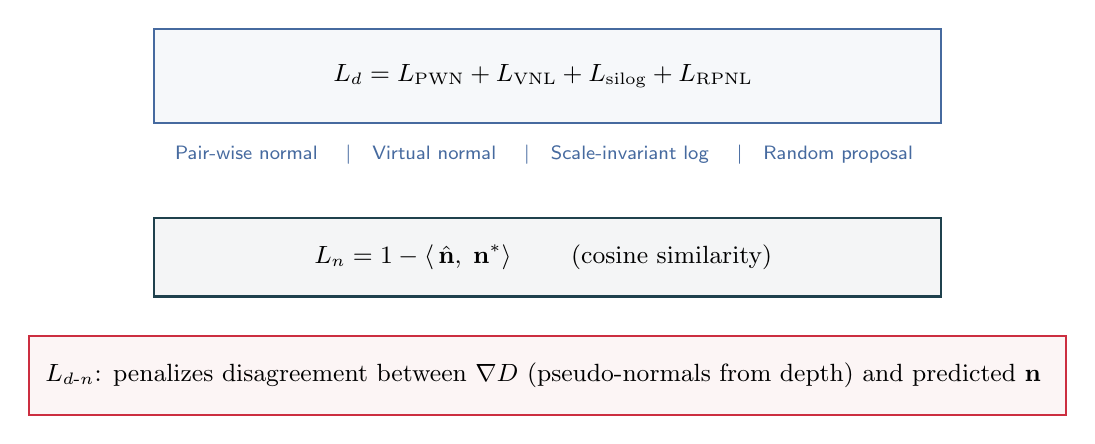
\begin{tikzpicture}
  % Depth losses
  \node[eqbox=atlantic, minimum width=10cm, minimum height=1.2cm] at (0,1.5) {
    $L_d = L_{\text{PWN}} + L_{\text{VNL}} + L_{\text{silog}} + L_{\text{RPNL}}$
  };
  \node[font=\scriptsize\sffamily, color=atlantic, align=center] at (0,0.5) {
    Pair-wise normal \quad$\mid$\quad Virtual normal \quad$\mid$\quad Scale-invariant log \quad$\mid$\quad Random proposal
  };

  % Normal loss
  \node[eqbox=congaree, minimum width=10cm, minimum height=1.0cm] at (0,-0.8) {
    $L_n = 1 - \langle\, \hat{\mathbf{n}},\; \mathbf{n}^{*} \rangle$
    \qquad (cosine similarity)
  };

  % Consistency loss
  \node[eqbox=rose, minimum width=10cm, minimum height=1.0cm] at (0,-2.3) {
    $L_{d\text{-}n}$: penalizes disagreement between $\nabla D$ (pseudo-normals from depth) and predicted $\mathbf{n}$
  };
\end{tikzpicture}

\vspace{0.3cm}
\textbf{Note:} $L_{d\text{-}n}$ weight is small (0.01) because pseudo-normals from predicted depth are noisy early in training. It acts as a gentle geometric regularizer.
\end{frame}

% ══════════════════════════════════════════════════════════
\section{Experiments}
% ══════════════════════════════════════════════════════════

% ── SLIDE 12: Training at Scale ───────────────────────────
\begin{frame}{Training at Scale}
\centering
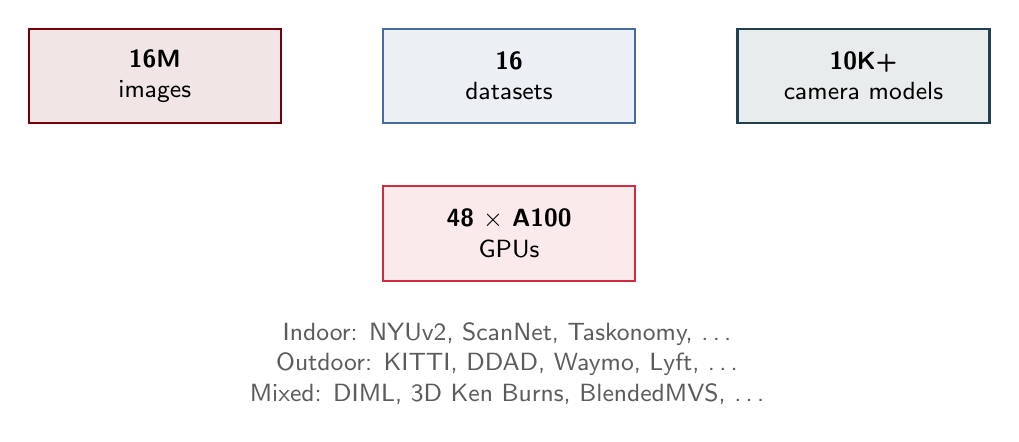
\begin{tikzpicture}
  % Stats boxes
  \node[pipeblock=garnet, minimum width=3.2cm, minimum height=1.2cm] (imgs) at (0,0)
    {\textbf{16M}\\images};
  \node[pipeblock=atlantic, minimum width=3.2cm, minimum height=1.2cm] (ds) at (4.5,0)
    {\textbf{16}\\datasets};
  \node[pipeblock=congaree, minimum width=3.2cm, minimum height=1.2cm] (cam) at (9,0)
    {\textbf{10K+}\\camera models};

  % GPU
  \node[pipeblock=rose, minimum width=3.2cm, minimum height=1.2cm] (gpu) at (4.5,-2)
    {\textbf{48 $\times$ A100}\\GPUs};

  % Annotation
  \node[font=\small\sffamily, color=bk70, below=0.4cm of gpu, align=center] {
    Indoor: NYUv2, ScanNet, Taskonomy, \ldots\\
    Outdoor: KITTI, DDAD, Waymo, Lyft, \ldots\\
    Mixed: DIML, 3D Ken Burns, BlendedMVS, \ldots
  };
\end{tikzpicture}

\vspace{0.5cm}
\textbf{Critical data gap:} Only $\sim$20K outdoor images have GT surface normals (mostly from ScanNet indoor).
This motivates the depth-normal consistency loss $L_{d\text{-}n}$ as a way to learn normals from depth-only outdoor data.
\end{frame}

% ── SLIDE 13: Benchmark Results ───────────────────────────
\begin{frame}{Benchmark Results}
\begin{columns}[T]
\column{0.55\textwidth}
\textbf{Zero-shot metric depth} (no fine-tuning on target dataset):

\vspace{0.2cm}
\begin{tabular}{lcc}
  \toprule
  \textbf{Dataset} & \textbf{AbsRel $\downarrow$} & \textbf{$\delta_1$ $\uparrow$} \\
  \midrule
  NYUv2 & \textcolor{garnet}{\textbf{0.063}} & \textcolor{garnet}{\textbf{0.975}} \\
  KITTI & \textcolor{garnet}{\textbf{0.043}} & \textcolor{garnet}{\textbf{0.989}} \\
  ScanNet & 0.069 & 0.970 \\
  DIODE Out & 0.308 & 0.832 \\
  \bottomrule
\end{tabular}

\vspace{0.3cm}
\textbf{Key:} Zero-shot results that \textit{beat} methods fine-tuned on the target dataset. CSTM enables generalization across camera types.

\column{0.42\textwidth}
% Placeholder for demo output
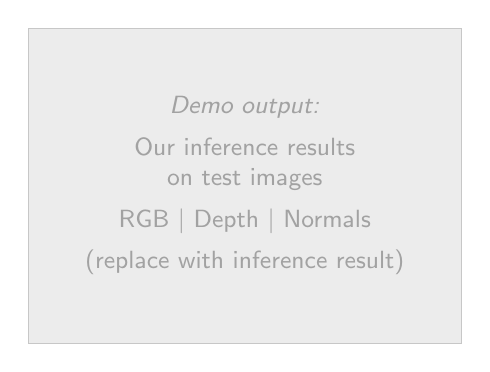
\begin{tikzpicture}
  \node[rectangle, draw=bk30, fill=bk10, minimum width=5.5cm, minimum height=4.0cm,
        font=\small\sffamily\color{bk50}, align=center] {
    \textit{Demo output:}\\[4pt]
    Our inference results\\
    on test images\\[4pt]
    RGB $\mid$ Depth $\mid$ Normals\\[4pt]
    (replace with inference result)
  };
\end{tikzpicture}
\end{columns}
\end{frame}

% ── SLIDE 14: Downstream Applications ────────────────────
\begin{frame}{Downstream Applications}
\begin{columns}[T]
\column{0.32\textwidth}
\textbf{3D Reconstruction}\\[4pt]
Back-project depth to point cloud:
\[
  X = \frac{(u - u_0) \cdot D}{f}
\]
\[
  Y = \frac{(v - v_0) \cdot D}{f}
\]
\[
  Z = D
\]

Table 6: competitive with MVS methods using a \textit{single} image.

\column{0.32\textwidth}
\textbf{SLAM Improvement}\\[4pt]
Using Metric3D v2 as depth prior in visual SLAM:
\begin{itemize}
  \item 10$\times$ reduction in drift (Table 7)
  \item Enables metric-scale monocular SLAM
\end{itemize}

\column{0.32\textwidth}
\textbf{Our Point Cloud Demo}\\[4pt]
% Placeholder for point cloud
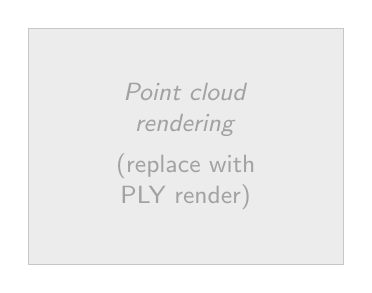
\begin{tikzpicture}
  \node[rectangle, draw=bk30, fill=bk10, minimum width=4cm, minimum height=3cm,
        font=\small\sffamily\color{bk50}, align=center] {
    \textit{Point cloud}\\
    \textit{rendering}\\[4pt]
    (replace with\\PLY render)
  };
\end{tikzpicture}
\end{columns}
\end{frame}

% ══════════════════════════════════════════════════════════
\section{Critical Comments}
% ══════════════════════════════════════════════════════════

% ── SLIDE 15: Strengths ──────────────────────────────────
\begin{frame}{Strengths}
\begin{enumerate}
  \item \textbf{CSTM is elegant and modular.} A single scaling factor $\omega = f^c / f$ handles all camera diversity. No architecture changes needed; works with any backbone.

  \vspace{0.2cm}
  \item \textbf{Learning normals from depth-only data.} The consistency loss $L_{d\text{-}n}$ sidesteps the scarcity of outdoor normal annotations ($\sim$20K images). The network learns normals as a \textit{byproduct} of depth prediction.

  \vspace{0.2cm}
  \item \textbf{Comprehensive evaluation.} Tested on 16+ benchmarks spanning indoor, outdoor, in-the-wild, and downstream tasks (3D reconstruction, SLAM, metrology).

  \vspace{0.2cm}
  \item \textbf{Immediately usable.} Available via PyTorch Hub with multiple model sizes (ViT-S, ViT-L, ViT-G). One line of code to run inference.
\end{enumerate}
\end{frame}

% ── SLIDE 16: Limitations ────────────────────────────────
\begin{frame}{Limitations and Open Questions}
\begin{enumerate}
  \item \textbf{Requires camera intrinsics at inference.} Unlike UniDepth (CVPR 2024) and Depth Pro (Apple, 2024), which estimate intrinsics internally. Users must provide or estimate $f$.

  \vspace{0.15cm}
  \item \textbf{Single-frame only.} No temporal consistency for video. Sequential frames can produce flickering depth maps.

  \vspace{0.15cm}
  \item \textbf{Outdoor normal data scarcity persists.} The consistency loss helps but does not fully close the gap; outdoor normal quality lags indoor.

  \vspace{0.15cm}
  \item \textbf{Canonical focal length $f^c = 1000$ is ad hoc.} The paper provides no theoretical justification for this choice. Sensitivity analysis would strengthen the claim.

  \vspace{0.15cm}
  \item \textbf{Newer competitors are closing the gap.}
    \begin{itemize}
      \item \textbf{MoGe} (CVPR 2025): jointly predicts 3D points + normals + FOV
      \item \textbf{Depth Pro}: metric depth without intrinsics at 0.3s per image
    \end{itemize}
\end{enumerate}
\end{frame}

% ══════════════════════════════════════════════════════════
\section{Conclusion}
% ══════════════════════════════════════════════════════════

% ── SLIDE 17: Takeaways ──────────────────────────────────
\begin{frame}{Key Takeaways}
\centering

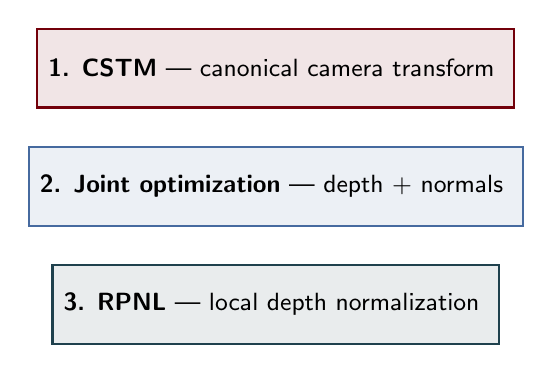
\begin{tikzpicture}[node distance=1.0cm]
  \node[pipeblock=garnet, minimum width=5cm, minimum height=1.0cm] (c1) at (0,2) {
    \textbf{1. CSTM} --- canonical camera transform
  };
  \node[pipeblock=atlantic, minimum width=5cm, minimum height=1.0cm] (c2) at (0,0.5) {
    \textbf{2. Joint optimization} --- depth + normals
  };
  \node[pipeblock=congaree, minimum width=5cm, minimum height=1.0cm] (c3) at (0,-1.0) {
    \textbf{3. RPNL} --- local depth normalization
  };
\end{tikzpicture}

\vspace{0.5cm}
\textbf{Big idea:} Transforming the \textit{data space} (CSTM) is simpler and more effective than encoding camera parameters into the network architecture.

\vspace{0.3cm}
Geometric foundation models trained on massive diverse data can rival --- and often beat --- task-specific models fine-tuned on individual benchmarks.

\vspace{0.5cm}
{\large\textcolor{garnet}{Questions?}}
\end{frame}

\end{document}
